\documentclass[tikz]{standalone}

\def\circRad{4em}

\begin{document}
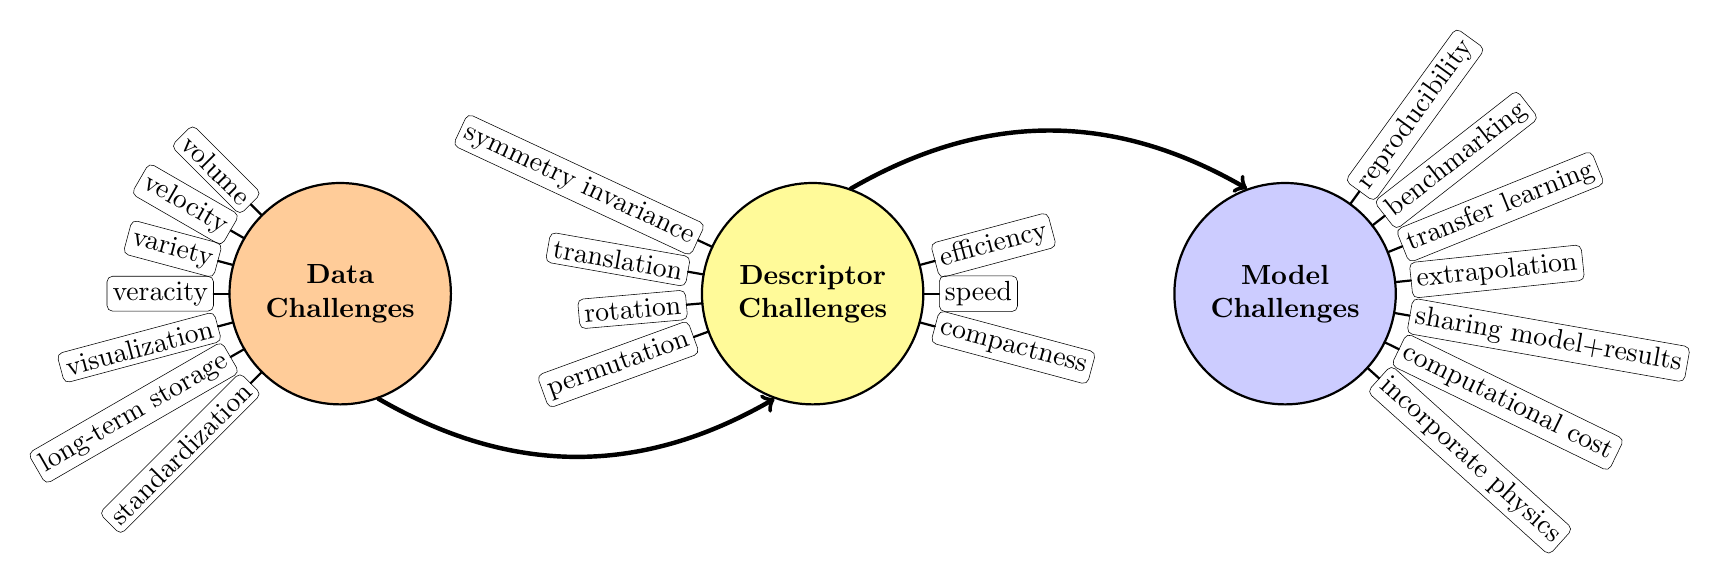
\begin{tikzpicture}[
    line cap=round, thick,
    stage/.style={shape=circle, draw, font=\bfseries, minimum width=2*\circRad},
    challenge/.style={draw, very thin, inner sep=2, rounded corners=2},
    every node/.style={align=center},
  ]

  \begin{scope}[local bounding box=challenges]
    % Data
    \node [stage, fill=orange!40] (data) {Data\\Challenges};
    \foreach \itm [count=\i, evaluate={\a=\i*15+120;}] in
      {volume, velocity, variety, veracity, visualization, long-term storage, standardization} {
        \node[challenge] at (\a:\circRad + 2mm) [rotate=\a+180, anchor=east] {\itm};
        \draw (\a:\circRad + 2mm) -- (\a:\circRad);
      }

    % Descriptor
    \begin{scope}[xshift=6cm]
      \node [stage, fill=yellow!40] (descriptor) {Descriptor\\Challenges};
      \foreach \itm [count=\i, evaluate={\a=\i*15+140;}] in
        {symmetry invariance, translation, rotation, permutation} {
          \node[challenge] at (\a:\circRad + 2mm) [rotate=\a+180, anchor=east] {\itm};
          \draw (\a:\circRad + 2mm) -- (\a:\circRad);
        }
      \foreach \itm [count=\i, evaluate={\a=30-\i*15;}] in
        {efficiency, speed, compactness} {
          \node[challenge] at (\a:\circRad + 2mm) [rotate=\a, anchor=west] {\itm};
          \draw (\a:\circRad + 2mm) -- (\a:\circRad);
        }
    \end{scope}

    % Model
    \begin{scope}[xshift=12cm]
      \node [stage, fill=blue!20] (model) {Model\\Challenges};
      \foreach \itm [count=\i, evaluate={\a=70-\i*16;}] in
        {reproducibility, benchmarking, transfer learning, extrapolation, {sharing model+results}, computational cost, incorporate physics} {
          \node[challenge] at (\a:\circRad + 2mm) [rotate=\a, anchor=west] {\itm};
          \draw (\a:\circRad + 2mm) -- (\a:\circRad);
        }
    \end{scope}
  \end{scope}

  \draw[ultra thick,->] (data.-70) to [bend right] (descriptor.-110);
  \draw[ultra thick,->] (descriptor.70) to [bend left] (model.110);

\end{tikzpicture}
\end{document}
